% -*- mode:flyspell; mode:latex -*-
\documentclass[12pt]{article}
\addtolength{\oddsidemargin} {-0.885in}
\addtolength{\textwidth}{1.75in}
\addtolength{\evensidemargin}{-0.8in}


\usepackage[latin1]{inputenc}
\usepackage[T1]{fontenc}
\usepackage[english]{babel}
\usepackage{graphicx}
\usepackage{float}


\usepackage{tikz}
\usepackage{[caption}
\usetikzlibrary{arrows}
\usetikzlibrary{decorations.markings}
\usetikzlibrary{decorations.pathmorphing}
% \usepackage[absolute,overlay]{textpos}
% \usepackage{onimage}

\usepackage{times}
\usepackage{graphics}

% \usepackage{subfigure}
% \usepackage{scalefnt}
%
% \renewcommand\thesubfigure{\arabic{subfigure}}

\usepackage{amsmath}
\usepackage{hyperref}
\usepackage{hhline}
\usepackage{subfig}
\usepackage{color}
\usepackage[all]{hypcap}

\usepackage[normalem]{ulem}  % for striking out
% \usepackage{fancyhdr}
% \pagestyle{fancy}
% \fancyhead[C]{}
% \fancyhead[L] {\it{Mu2e-doc-29670-v1.0} }
%%%%%%%%%%%%%%%%%%%%%%%%%%%%%%%%%%%%%%%%%%%%%%%%%%%%%%%%%%%%%%%%%%%%%%%%%%%%%%
% use natbib - biblatex not available on Mu2e interactive nodes
%%%%%%%%%%%%%%%%%%%%%%%%%%%%%%%%%%%%%%%%%%%%%%%%%%%%%%%%%%%%%%%%%%%%%%%%%%%%%%
\usepackage[square,sort,comma,numbers]{natbib}

% location of the .bib files: env var BIBINPUTS (~/library/bibliography)

% \usepackage[backend=biber, style=numeric-comp, sorting=ynt] {biblatex}
% \addbibresource{clfv.bib}

% \addbibresource{stntuple.bib}
% \addbibresource{mu2e_web.bib}
% \addbibresource{radiative_pion_capture.bib}

\graphicspath{{figures/}}
%%%%%%%%%%%%%%%%%%%%%%%%%%%%%%%%%%%%%%%%%%%%%%%%%%%%%%%%%%%%%%%%%%%%%%%%%%%%%%
% for portability, make sure all commands are included locally
% order them alphabetically
%%%%%%%%%%%%%%%%%%%%%%%%%%%%%%%%%%%%%%%%%%%%%%%%%%%%%%%%%%%%%%%%%%%%%%%%%%%%%%
% \include{commands}

\newcommand {\keVc}       {\mbox{$\rm keV\!/\!c$}}
\newcommand {\kmax}       {\mbox{$k_{\rm max}$}}

\newcommand {\MeVc}       {\mbox{$\rm MeV\!/\!c$}}
\newcommand {\MeVcsq}     {\mbox{$\rm MeV\!/\!c^2$}}

\newcommand {\mumemconv}[1][A] {\mbox{$\mu^- \textrm{#1} \rightarrow e^- \textrm{#1}$}}
% Define a relay to have 2 default arguments instead of limit of 1
\newcommand {\mumepconv}[1][A] {%
  \def\ArgI{{#1}}%store the first argument
  \mumepconvRelay
}
\newcommand \mumepconvRelay[1][A]  {\mbox{$\mu^- \textrm{\ArgI} \rightarrow e^+ \textrm{#1}$}}
\newcommand {\MuToEm}     {\mbox{$\mu^- \ra e^-$}}
\newcommand {\MuToEp}     {\mbox{$\mu^- \ra e^+$}}
\newcommand {\MuPToEp}    {\mbox{$\mu^+ \ra e^+$}}
\newcommand {\ra}        {\rightarrow}
\newcommand {\tandip}    {\mbox{$\tan \lambda$}}

\newcommand {\Pb}[1]     {\mbox{$\rm ^{#1}Pb$}}                 % isotopes of lead
\newcommand {\Au}[1]     {\mbox{$\rm ^{#1}Au$}}                 % isotopes of gold
\newcommand {\Ir}[1]     {\mbox{$\rm ^{#1}Ir$}}                 % isotopes of iridium
%%%%%%%%%%%%%%%%%%%%%%%%%%%%%%%%%%%%%%%%%%%%%%%%%%%%%%%%%%%%%%%%%%%%%%%%%%%%%%
% editing commands
%%%%%%%%%%%%%%%%%%%%%%%%%%%%%%%%%%%%%%%%%%%%%%%%%%%%%%%%%%%%%%%%%%%%%%%%%%%%%%
\newcommand {\add}[1]    {{\red #1}}
\newcommand {\alt}[1]    {{\green #1}} %alternate comment color
\newcommand {\del}[1]    {{\blue \sout{#1}}}
\newcommand {\dlt}[1]    {{\violet \sout{#1}}} %alternate delete color

\newcommand {\black}     {\color{black}}
\newcommand {\red}       {\color{red}}
\newcommand {\blue}      {\color{blue}}
\newcommand {\strike}[1] {{\blue \sout{#1}}}
%%%%%%%%%%%%%%%%%%%%%%%%%%%%%%%%%%%%%%%%%%%%%%%%%%%%%%%%%%%%%%%%%%%%%%%%%%%%%%
\begin{document}

\begin{titlepage}
  \begin{flushright}
    \bf {MU2E/PHYSICS/40523} \\
    version 1.05
    \today
 \end{flushright}

  \vspace{1cm}

  \begin{center}
    {\Large \bf Mu2e 2020 sensitivity update.

      \vspace{0.3in}

      11. Estimate of the beam backgrounds
    }

    \vspace{1cm}

    P. Murat(FNAL)

    % \footnote{\texttt{Fermilab; e-mail: murat@fnal.gov}}
    \vspace{0.3cm}

    \vspace{0.8cm}
  \end{center}

  \begin{abstract}
    This note presents an estimate of the beam electron background in \MuToEm\ channel
    for the Mu2e 2020 sensitivity update (SU2020).
    \vspace{0.2in}
  \end{abstract}

\end{titlepage}
% \frontmatter
% \chapter*{Abstract}
%
% \addcontentsline{toc}{chapter}{Abstract}
%
% \mainmatter
%
{\tableofcontents}

%%%%%%%%%%%%%%%%%%%%%%%%%%%%%%%%%%%%%%%%%%%%%%%%%%%%%%%%%%%%%%%%%%%%%%%%%%%%%%%
%\chapter{Calibration}
%%%%%%%%%%%%%%%%%%%%%%%%%%%%%%%%%%%%%%%%%%%%%%%%%%%%%%%%%%%%%%%%%%%%%%%%%%%%%%%
% \input{input_data}

%%%%%%%%%%%%%%%%%%%%%%%%%%%%%%%%%%%%%%%%%%%%%%%%%%%%%%%%%%%%%%%%%%%%%%%%%%%%%%%
\newpage
\section {Revision history}
\begin{itemize}
\item
  v1.01: initial version
\end{itemize}

%%%%%%%%%%%%%%%%%%%%%%%%%%%%%%%%%%%%%%%%%%%%%%%%%%%%%%%%%%%%%%%%%%%%%%%%%%%%%%
\section {Introduction}

In this note, we discuss several small beam-associated backgrounds, not related to
the muon stops in the stopping target. They could be split into three categories:

\begin{itemize}
\item 
  P>100 electrons scattering in the stopping target and producing reconstructed tracks
\item
  $\mu^- \ra e^- \nu \nu$ decays in flight after the stopping target producing p>100 \MeVc\
  electrons reconstructed in the detector
\item
  beam muons with P > 100 \MeVc\ scattered at a large angle in the ST, reconstructed in the detector
  and mis-identified as P > 100 \MeVc\ electrons 
\end{itemize}

As it takes a 100 \MeVc\ particle ~100-200 ns to travel from the production target to DS and
traverse the detector, ``in-time'' protons, arriving at the production target in pulses, 
do not contribute. The contributions from all three sources are due to the ``out-of-time''
protons arriving at the production target in between the proton pulses and suppressed by the
extinction system. According to the Mu2e technical requirements, the proton beam extinction
factor $f_{ext} < 10^{-10}$.

Contributions of all sources above are expected to be small.

Existing Mu2e estimates of the background from beam electrons and decays in flight
were making assumptions which need validation - that will be discussed in the corresponding sections.

Contribution of the muon scattering is suppressed by the particle identification, however the
muon mis-ID rate of $10^{-2} - 10^{-3} $in the stopping target so far has been neglecte

There are $\sim$ 100 \MeVc\ electrons entering the DS. There are several source of those:
\begin{itemize}
\item
  electrons produced by $\pi^0$ . THose are entering the TS and need to make it through
\item
  muon decays in flight - happen all over
\end{itemize}

To produce a 100 MeV/c electron, a muon has to have a lower momentum.

Thus - higher transport efficiency. Can't resample uniformly.

To make a track, an electron has to scatter in the ST.

Also: muon decays inside the DS producing an electron which track gets reconstructed.

%%%%%%%%%%%%%%%%%%%%%%%%%%%%%%%%%%%%%%%%%%%%%%%%%%%%%%%%%%%%%%%%%%%%%%%%%%%%%%
\section {Simulation strategy}

Trace events till the VD9. At that point, select events with P>100 MeV/c electrons.
Resample by a needed factor.
Keep in mind that the probability to scatter and make hits in the tracker is $< 1 \times 10^{-5}$.
Therefore, starting from VD9, need to run at least $10^6$ events.

As the goal is to produce an upper bound, try not to run reconstruction, just the simulation.
It might work.

Simulation stages:

\begin{itemize}
\item
  Stage1 : proton interactions in the production target --> before TS31 collimator 
\item
  Stage2 : before TS31 collimator -> before TS5 collimator
\item
  Stage3 : before TS5 collimator --> VD9
\item
  Stage4 : before VD9 --> tracker mother volume
\item
  Stage5 : hit simulation, digitization. Count events with 20+ hits produced by a 100 MeV/c+ electron
\end{itemize}

\begin{itemize}
\item [stage 1]
  generate $1 \times 10^9$ POT, output of stage 1: bmum0s11b0
\item
  to reduce computing effort,
  after stage 1, strip events with muons P > 70 MeV/c : bmum0s1b. 
  Only these may produce 100 MeV/c electrons
\item
  after stage 1, strip events with electrons P > 100 MeV/c : bmum0s16b0. Trace these events separately:
  \begin{itemize}
  \item
    after stage2: bmum0s26b0
  \item
    after stage3: (TS5-->VD9): bmum0s36b0
  \end{itemize}
\item
  trace the rest events through stage2: bmum0s27b0
  \begin{itemize}
  \item
    strip events with electrons: bmum0s28b0 (these should be muon decay in flights only)
  \end{itemize}
\item
  trace bmum0s28b0 as electrons to VD9 :  bmum0s38b0
\item
  trace (bmum0s27b0 minus bmum0s28b0) to VD9 : bmum0s37b0
\item
  strip events with electrons to bmum0s39b0
\item
  bmum0s36b0 (pi0 + mu decays at S1) + bmum0s38b0 (mu decays at S2) + bmum0s39b0 (mu decays at S3) : electrons at VD9.
\item
  trace bmum0s37b0 minus bmum0s29b0) to VD10 : bmum0s47b0.
  strip events with electrons : bmum0s4ab0. (muon decays at S4) - assume the probability of
  scattering in the target is not larger than for electrons from previous strips.
\item
  now need to trace muons, forcing decays before the calorimeter - how to do that ? 
\end{itemize}

 VD10 check 


\begin{table}[H]
  { \renewcommand{\arraystretch}{1.0}   % change 1.0 to 1.1 to increase the spacing between the table lines
    \begin{center}
      \begin{tabular}{|c|c|c|}
        \hline
        dataset ID   & N generated events  &  brief description                  \\
        \hline
        cele0s51b0   &  1,000,000          &  \MuToEm\  single particle dataset  \\
        cele0s61b1   &  1,000,000          &  \MuToEm\  + one-batch mode pileup    \\
        cele0s61b2   &  1,000,000          &  \MuToEm\  + two-batch mode pileup    \\
        \hline
        cpos0s51b0   &  1,000,000          &  \MuToEp\  single particle dataset  \\
        cpos0s61b1   &  1,000,000          &  \MuToEp\  + one-batch mode pileup    \\
        \hline
      \end{tabular}
    \end{center}
  }
  \caption{
    \label{tab:datasets}
    SU2020 signal datasets
  }
\end{table}


%%%%%%%%%%%%%%%%%%%%%%%%%%%%%%%%%%%%%%%%%%%%%%%%%%%%%%%%%%%%%%%%%%%%%%%%%%%%%%

\section {Beam electrons}

Traced down to VD9, resampled by x$10^4$.

\begin{itemize}
\item 
  electrons from S1: no candidate events, all electrons - very small pT
\item
  electrons from muon decays at Stage2:  no candidate events with P>100 \MeVc\ electrons entering 
  the tracker fiducial
\item
  electrons from muon decays at Stage3: 1 event candidate
\end{itemize}

For Run1 : N  = $4 \times 10^{19} \times 10^{-10} \times 10^{-9} \times 10^{-4}  ~=~ 4 \times 10^{-4}$


Electrons produced at Stage 1, in the end of Stage1 and Stage 2:

\begin{figure}[H]
  \hspace{-0.8in}
  \begin{tikzpicture}
    \node[anchor=south west,inner sep=0] at (0,0.) {
      % \node[shift={(0 cm,0.cm)},inner sep=0,rotate={90}] at (0,0) {}
      \makebox[\textwidth][c] {
        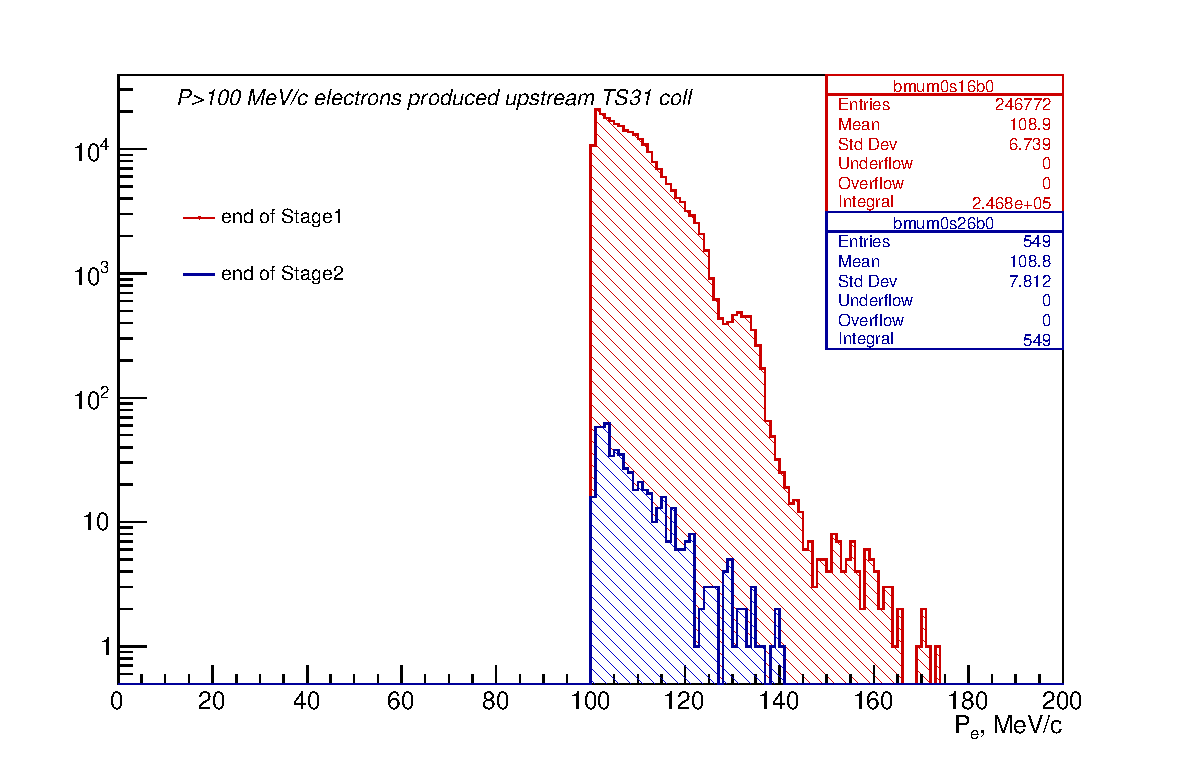
\includegraphics[width=0.8\textwidth]{figures/pdf/figure_00160_bmum0s16b0_vdet_102_mom}
      }
    };
  \end{tikzpicture}
  \caption{
    \label{fig:bmum0s16b0_momentum}
    Electrons produced before the end of Stage 1 
  }
\end{figure}

\begin{figure}[th]
  \hspace{-0.8in}
  \begin{tikzpicture}
    \node[anchor=south west,inner sep=0] at (0,0.) {
      % \node[shift={(0 cm,0.cm)},inner sep=0,rotate={90}] at (0,0) {}
      \makebox[\textwidth][c] {
        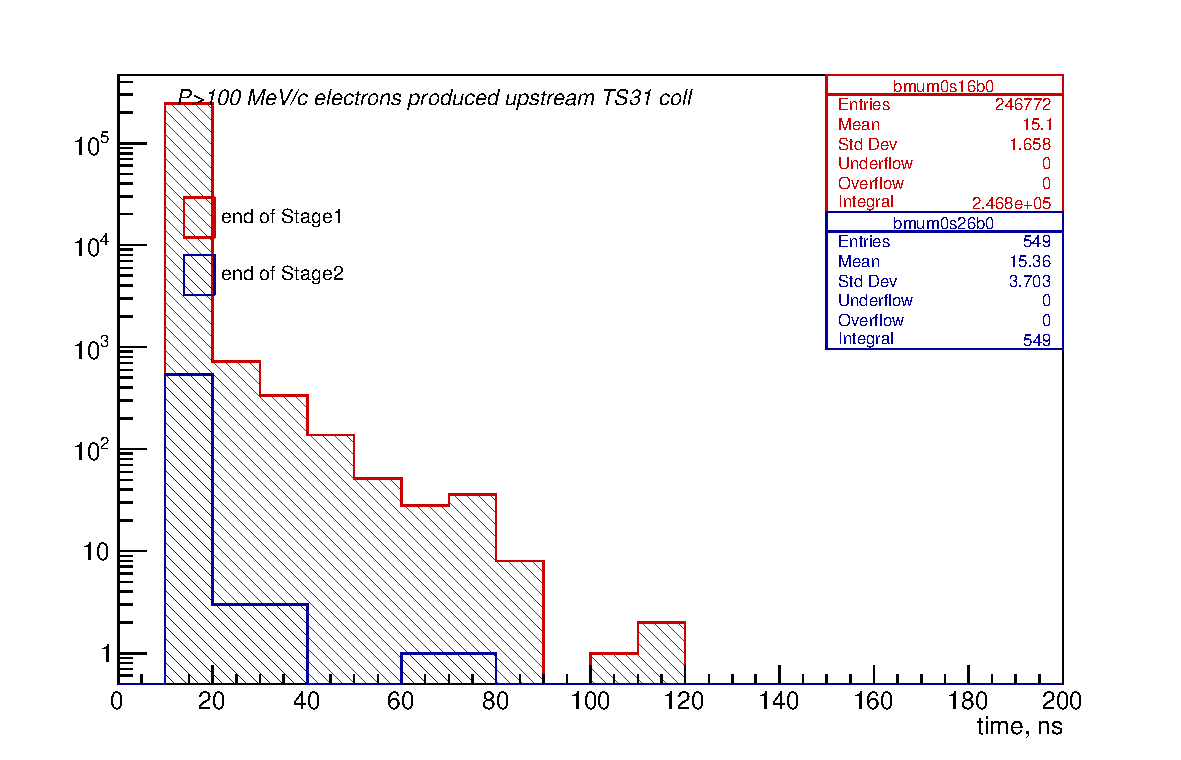
\includegraphics[width=0.8\textwidth]{figures/pdf/figure_00161_bmum0s16b0_vdet_102_time}
      }
    };
  \end{tikzpicture}
  \caption{
    \label{fig:bmum0s16b0_momentum}
    Electrons produced before the end of Stage 1 
  }
\end{figure}


In the end of stage2:

\begin{figure}[H]
  \hspace{-0.8in}
  \begin{tikzpicture}
    \node[anchor=south west,inner sep=0] at (0,0.) {
      % \node[shift={(0 cm,0.cm)},inner sep=0,rotate={90}] at (0,0) {}
      \makebox[\textwidth][c] {
        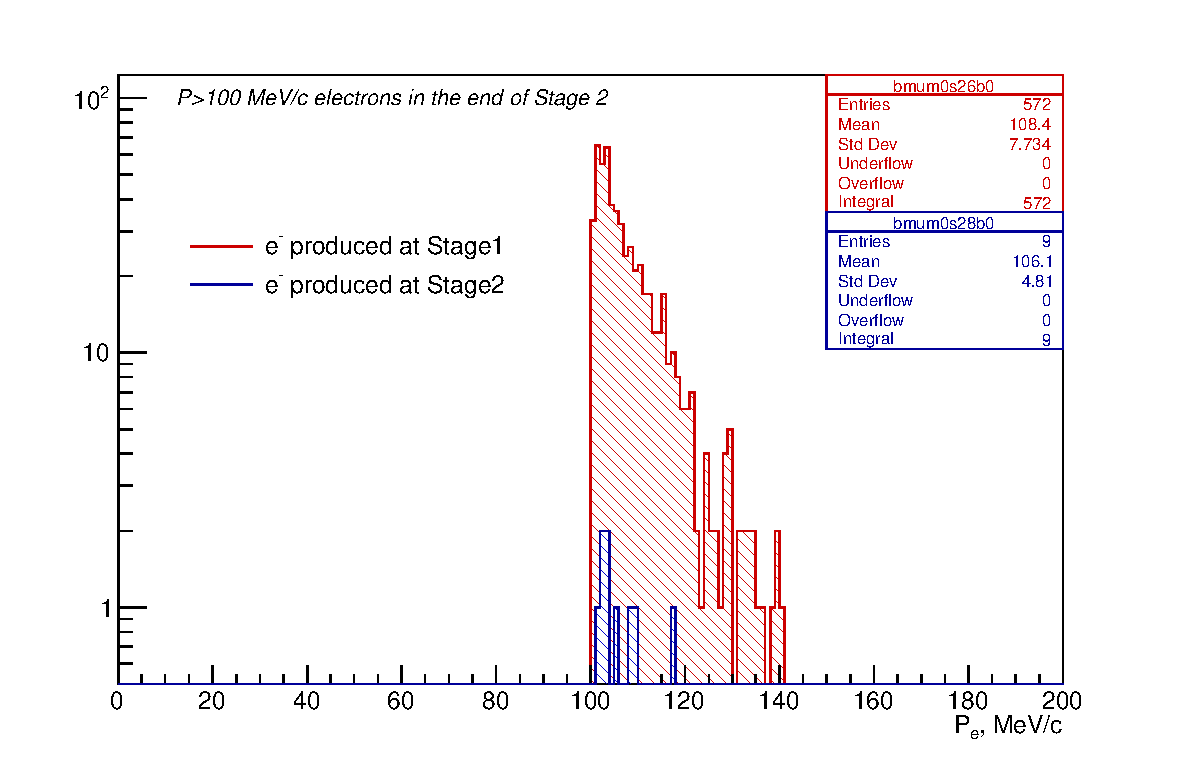
\includegraphics[width=0.8\textwidth]{figures/pdf/figure_00260_bmum0s26b0_vdet_106_mom}
      }
    };
  \end{tikzpicture}
  \caption{
    \label{fig:bmum0s26b0_momentum}
    Electrons produced before the end of Stage 1 
  }
\end{figure}

\begin{figure}[H]
  \hspace{-0.8in}
  \begin{tikzpicture}
    \node[anchor=south west,inner sep=0] at (0,0.) {
      % \node[shift={(0 cm,0.cm)},inner sep=0,rotate={90}] at (0,0) {}
      \makebox[\textwidth][c] {
        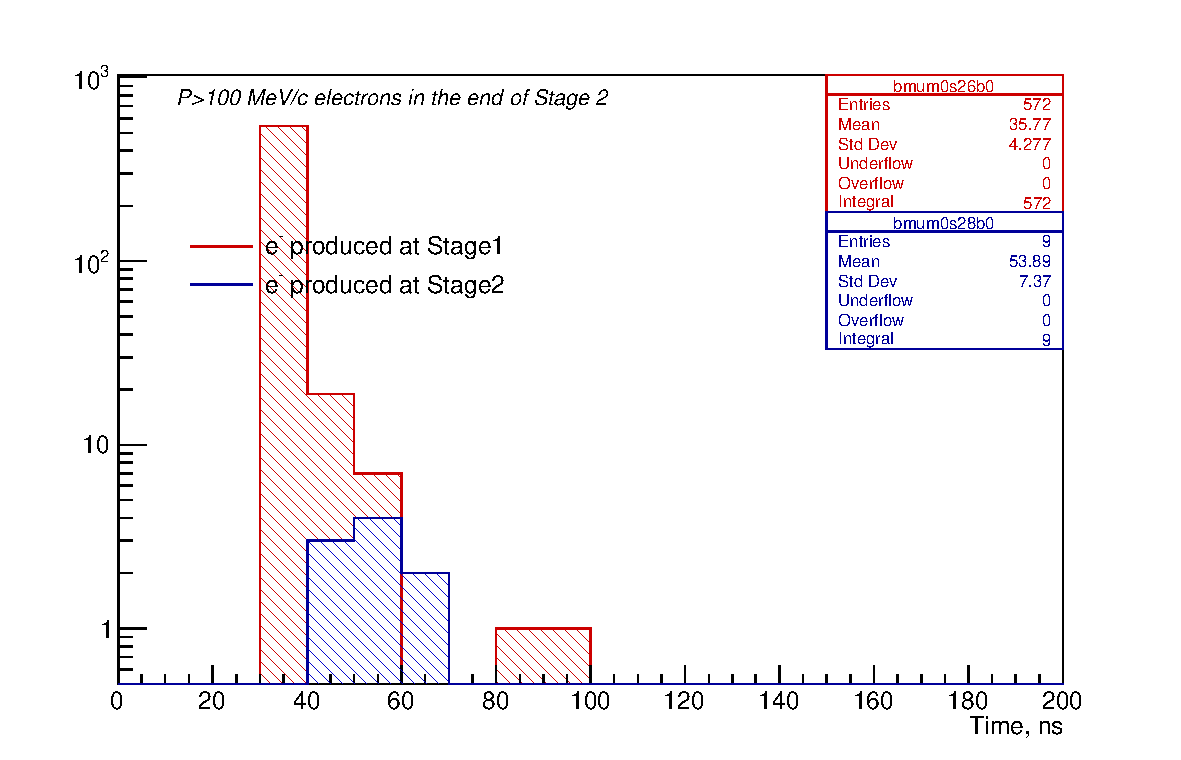
\includegraphics[width=0.8\textwidth]{figures/pdf/figure_00261_bmum0s26b0_vdet_106_time}
      }
    };
  \end{tikzpicture}
  \caption{
    \label{fig:bmum0s26b0_time}
    Electrons produced at Stage2 , time
  }
\end{figure}

%%%%%%%%%%%%%%%%%%%%%%%%%%%%%%%%%%%%%%%%%%%%%%%%%%%%%%%%%%%%%%%%%%%%%%%%%%%%%%
\subsection {Electrons Entering the Detector Envelope}

Resample electrons at VD9 by $10^4$, count events with electrons entering the detector envelope volume.

Assume flat distribution between 102 and 115 MeV/c, the signal window of 1.5 MeV/c.
Beam extinction of $1 \times 10^{-10}$, Normalize to $4 \times 10^{19}$ protons on target (POT):
$$
              N ~=~ 23/13 \times 1.5 \times 4 \times 10^{19} ({\rm N_{POT}}) \times 10^{-10}  ({\rm extinction}) / 10^{13} ({\rm statistics}) ~\simeq ~ 1 \times 10^{-3}
$$

The number is consistent with the TDR estimate \cite{MU2E_6464_CD3_BEAM_ELECTRONS}.
However we observe that the beam electron background is dominated by the electrons coming
from muon decays in flight in TSd and DS, after the TS3 collimator.
This contribution should not be sensitive to vertical misalignments,
and, in particular, to small variations of the PS magnetic field.

A lower estimate from 

\begin{figure}[H]
  \hspace{-0.8in}
  \begin{tikzpicture}
    \node[anchor=south west,inner sep=0] at (0,0.) {
      % \node[shift={(0 cm,0.cm)},inner sep=0,rotate={90}] at (0,0) {}
      % \makebox[\textwidth][c] {
      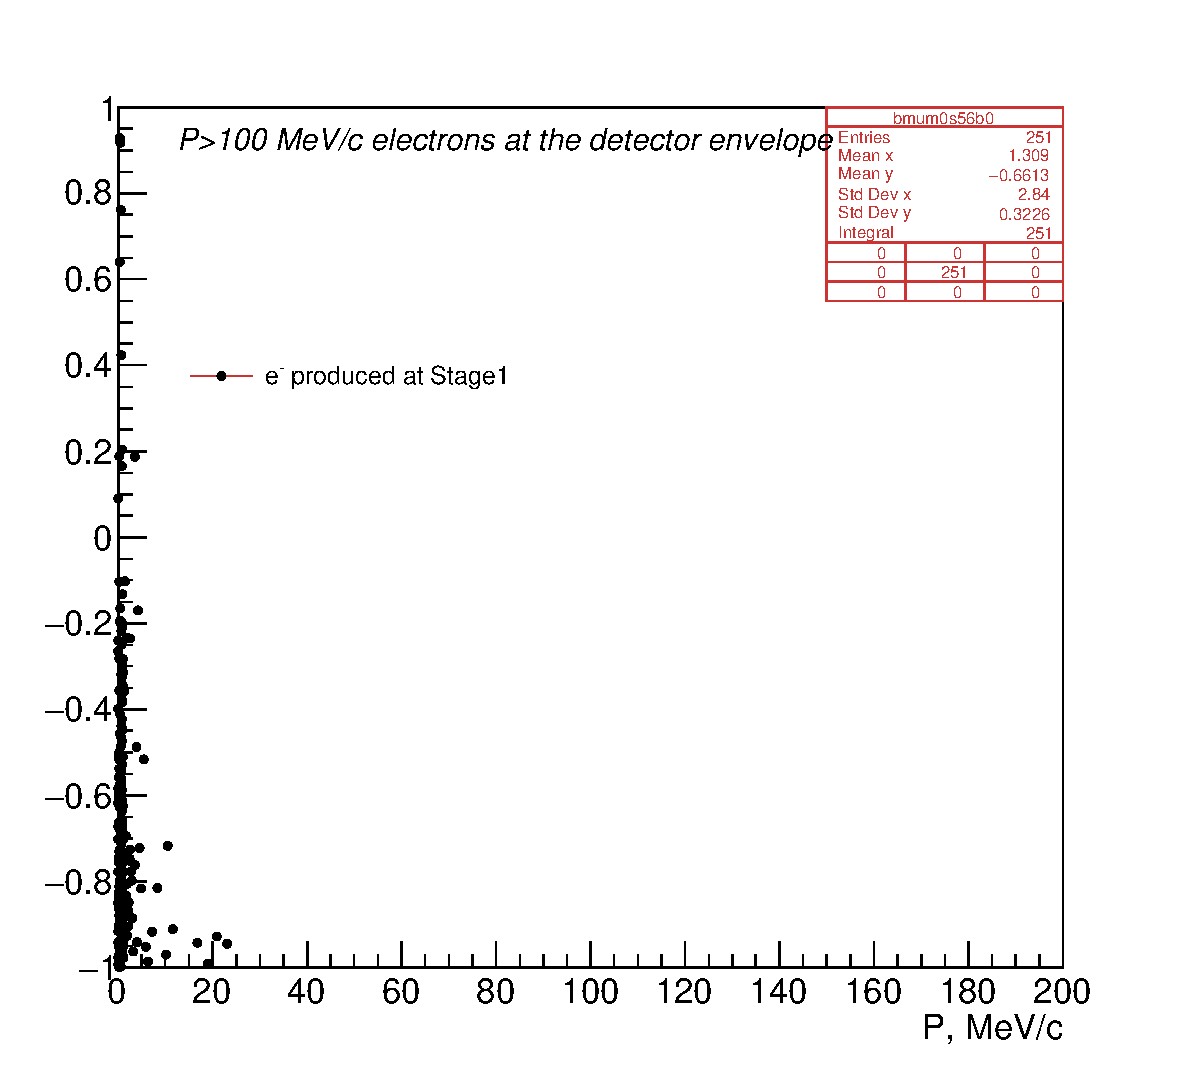
\includegraphics[width=0.54\textwidth]{figures/pdf/figure_00560_bmum0s56b0_spmc_1_cth_vs_mom_1}
      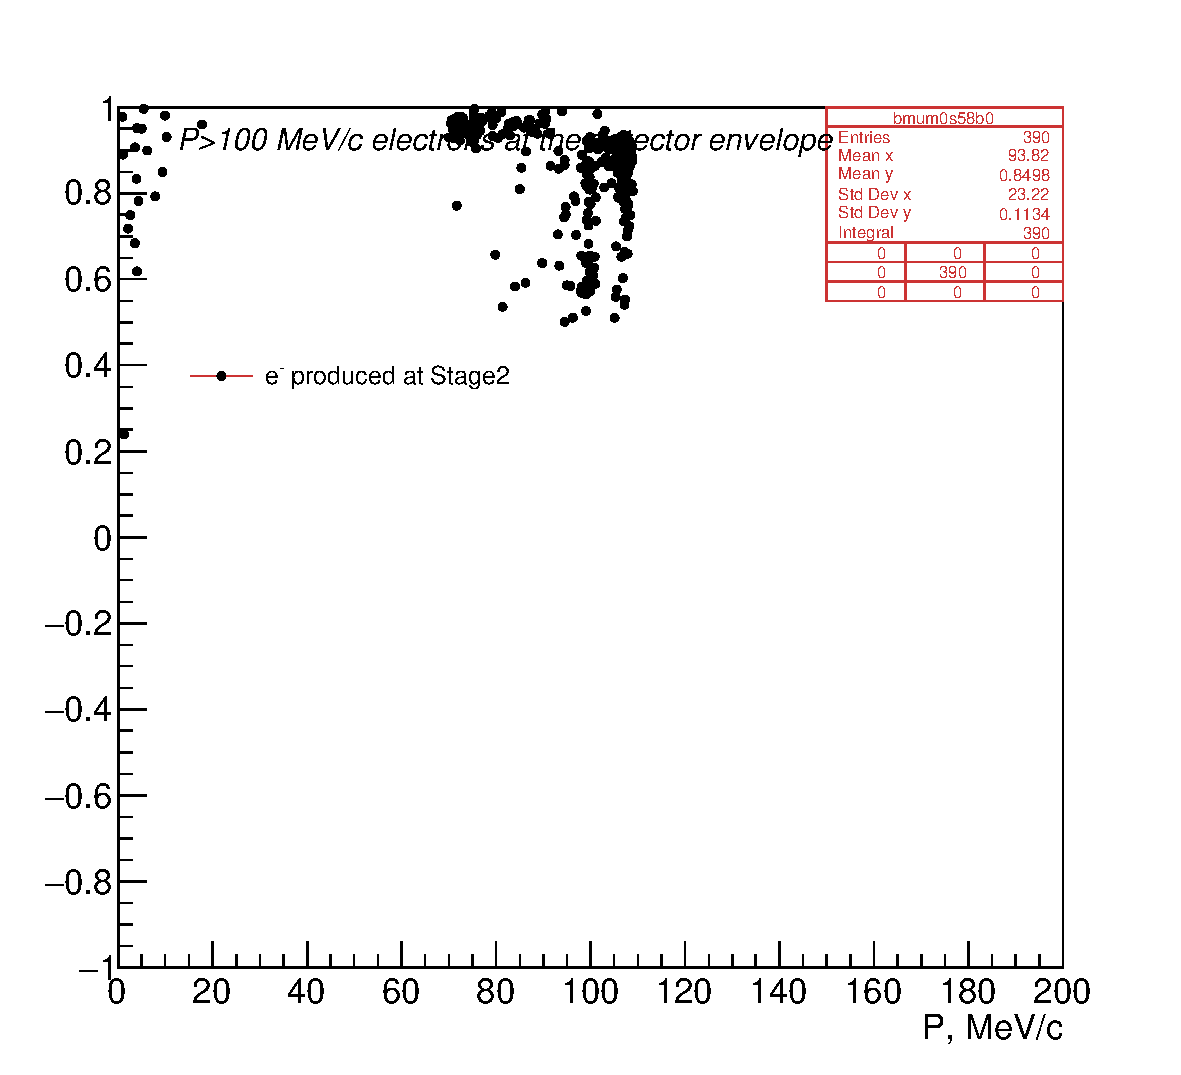
\includegraphics[width=0.54\textwidth]{figures/pdf/figure_00580_bmum0s58b0_spmc_1_cth_vs_mom_1}
      % }
    };
    \node[anchor=south west,inner sep=0] at (0,-10.) {
      % \node[shift={(0 cm,0.cm)},inner sep=0,rotate={90}] at (0,0) {}
      % \makebox[\textwidth][c] {
      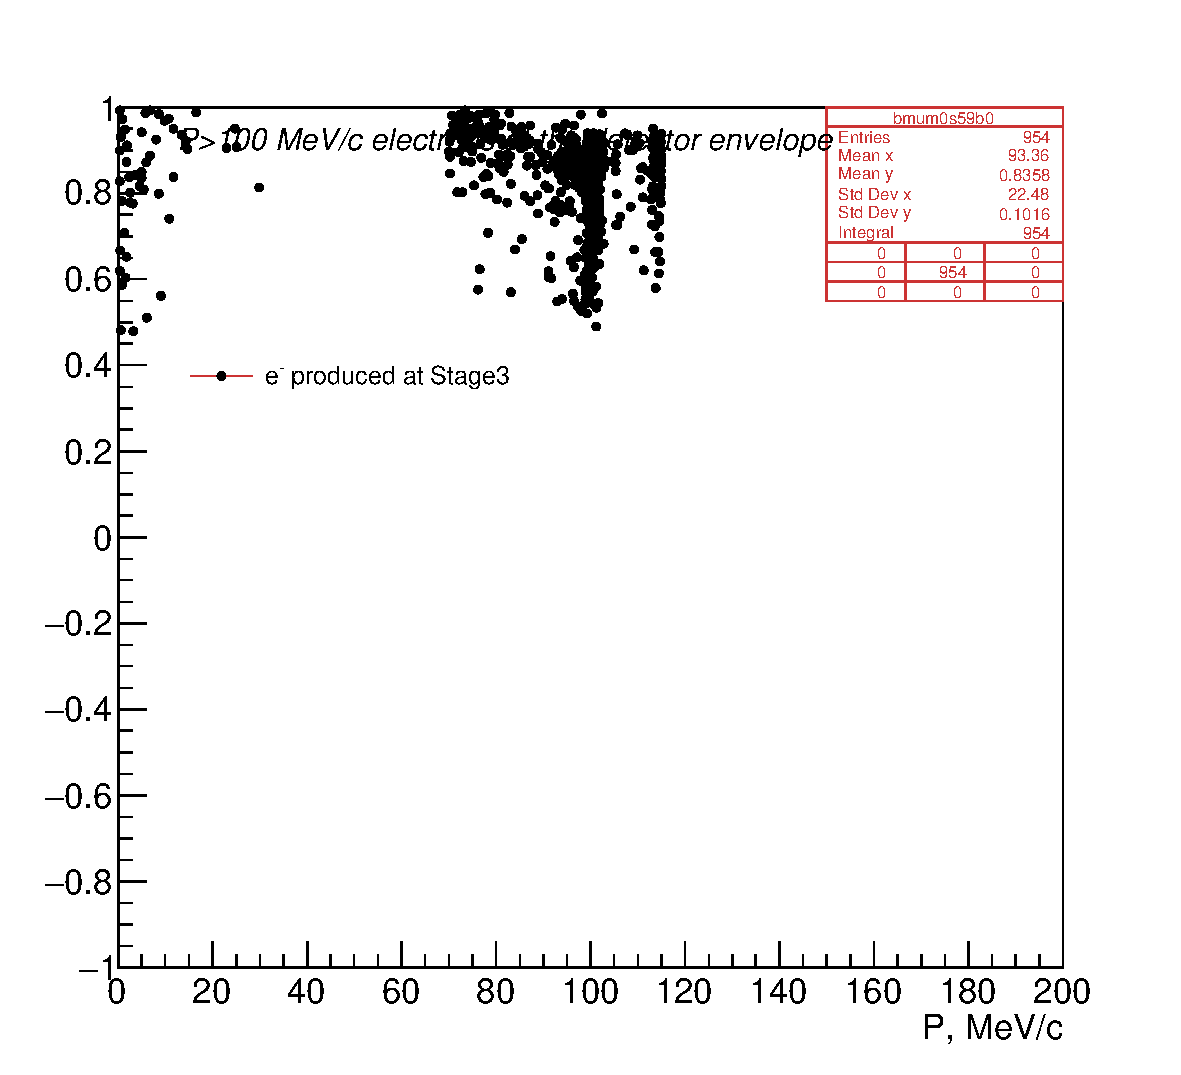
\includegraphics[width=0.54\textwidth]{figures/pdf/figure_00590_bmum0s59b0_spmc_1_cth_vs_mom_1}
      % }
    };
  \end{tikzpicture}
  \caption{
    \label{fig:bmum0s58b0_crt_vs_mom}
    Electrons entering the detector envelope
  }
\end{figure}

``Reconstruction'' : Selection of events with electrons P>100 MeV/c, cos(th) < 1./sqrt(2) - emulate
the reconstruction acceptance cuts.
\begin{figure}[H]
  \hspace{-0.8in}
  \begin{tikzpicture}
    \node[anchor=south west,inner sep=0] at (0,0.) {
      % \node[shift={(0 cm,0.cm)},inner sep=0,rotate={90}] at (0,0) {}
      % \makebox[\textwidth][c] {
      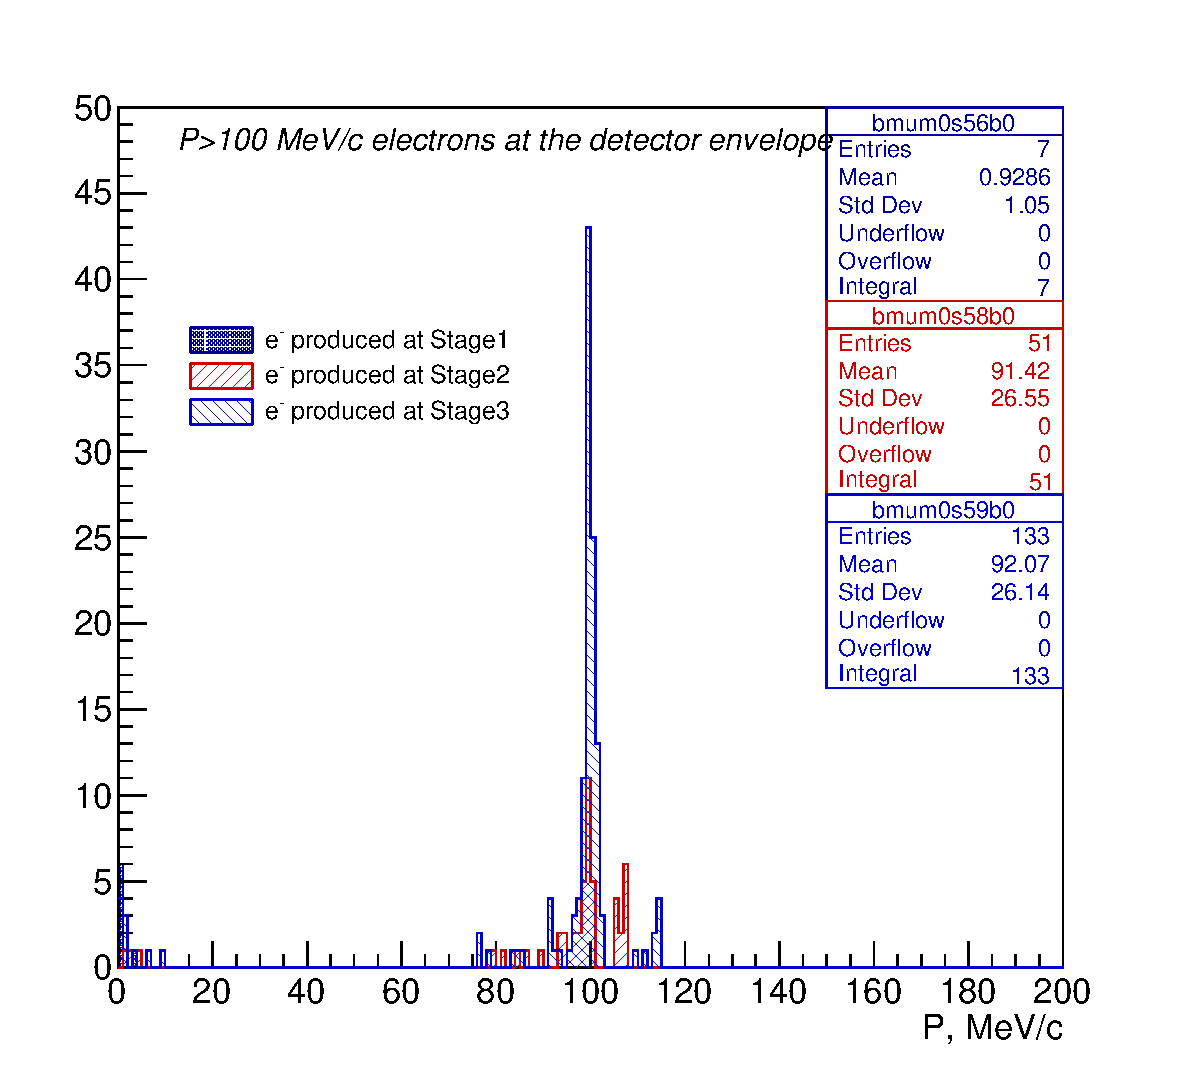
\includegraphics[width=0.54\textwidth]{figures/pdf/figure_01561_bmum0s59b0_spmc_1_mom}
      % }
    };
    \node[anchor=south west,inner sep=0] at (10,0.) {
      % \node[shift={(0 cm,0.cm)},inner sep=0,rotate={90}] at (0,0) {}
      % \makebox[\textwidth][c] {
      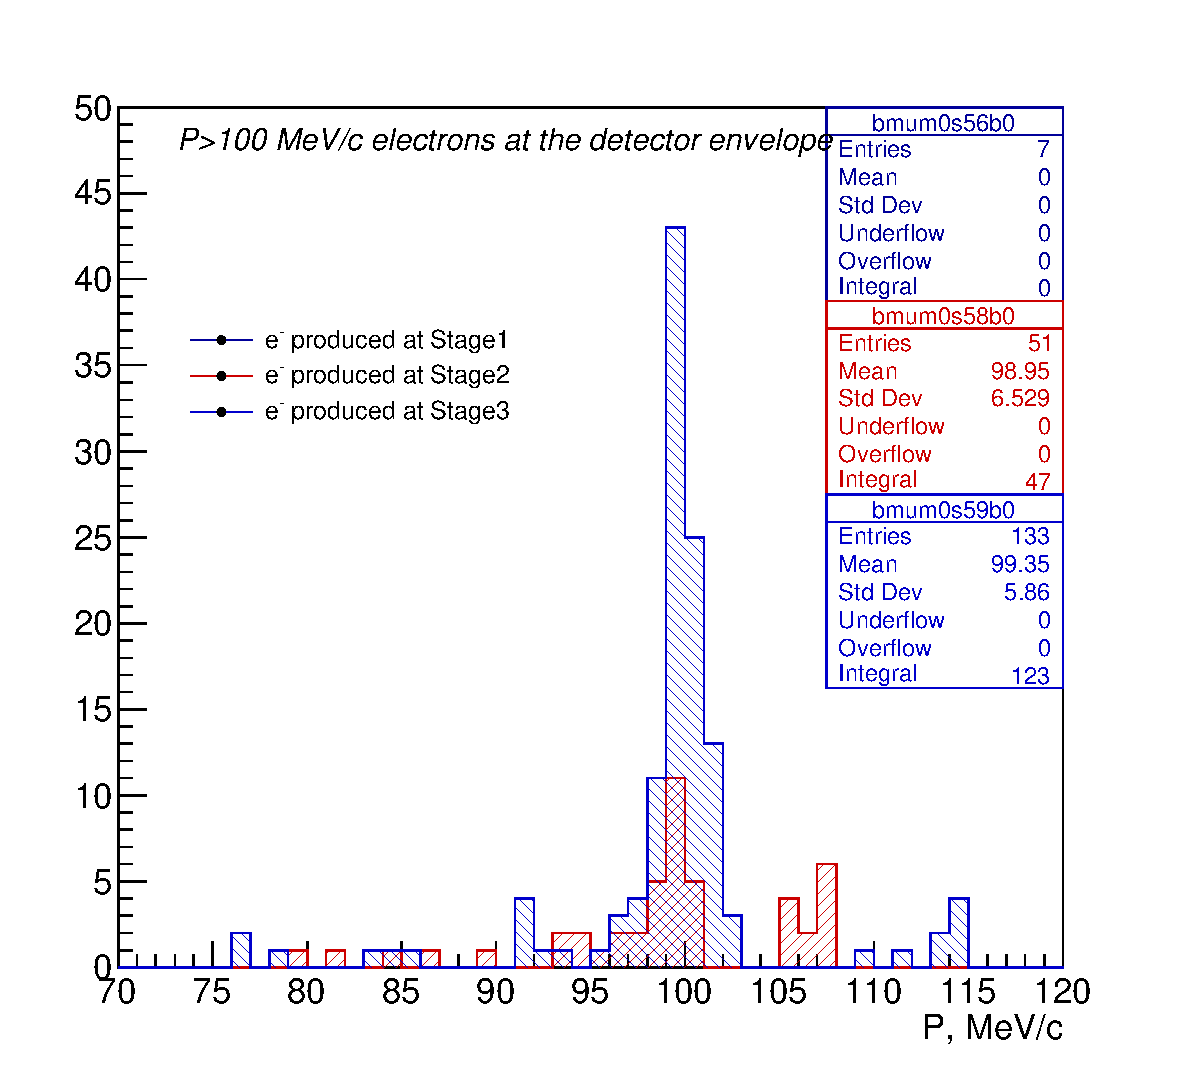
\includegraphics[width=0.54\textwidth]{figures/pdf/figure_01562_bmum0s59b0_spmc_1_mom}
      % }
    };
  \end{tikzpicture}
  \caption{
    \label{fig:bmum0s58b0_crt_vs_mom}
    Electrons entering the detector envelope
  }
\end{figure}


%%%%%%%%%%%%%%%%%%%%%%%%%%%%%%%%%%%%%%%%%%%%%%%%%%%%%%%%%%%%%%%%%%%%%%%%%%%%%%
\section {Muon decays in flight}

CD3 estimate: \cite{MU2E_4342_MUON_DECAYS_IN_FLIGHT_TDR}


%%%%%%%%%%%%%%%%%%%%%%%%%%%%%%%%%%%%%%%%%%%%%%%%%%%%%%%%%%%%%%%%%%%%%%%%%%%%%%
\section {Muon scattering in the ST}

% Figure \ref{fig:cele0s61b1_momentum} and Figure \ref{fig:tid_variables_cele0s61b1} show the
% reconstructed track momentum distribution and distributions of the track ID variables
% for {\bf cele0s61b1} dataset.
% 
% \begin{figure}[H]
%   \hspace{-0.8in}
%   \begin{tikzpicture}
%     \node[anchor=south west,inner sep=0] at (0,0.) {
%       % \node[shift={(0 cm,0.cm)},inner sep=0,rotate={90}] at (0,0) {}
%       \makebox[\textwidth][c] {
%         \includegraphics[width=0.8\textwidth]{figures/pdf/figure_00301_cele0s61b1_su2020_track_ana_trk_10_p}
%       }
%     };
%   \end{tikzpicture}
%   \caption{
%     \label{fig:cele0s61b1_momentum}
%     Track momentum distribution for the \MuToEm\ electrons + one-batch pileup dataset, {\bf cele0s61b1}.
%     Hashed region shows the benchmark momentum window.
%   }
% \end{figure}
% 
% \begin{figure}[H]
%   \hspace{-0.8in}
%   \begin{tikzpicture}
%     \node[anchor=south west,inner sep=0] at (0,0.) {
%       % \node[shift={(0 cm,0.cm)},inner sep=0,rotate={90}] at (0,0) {}
%       % \makebox[\textwidth][c] {
%       \includegraphics[width=0.64\textwidth]{figures/pdf/figure_00302_cele0s61b1_su2020_track_ana_tid_1_tandip}
%       % }
%     };
%     \node[anchor=south west,inner sep=0] at (10.7,0.) {
%       % \node[shift={(0 cm,0.cm)},inner sep=0,rotate={90}] at (0,0) {}
%       % \makebox[\textwidth][c] {
%       \includegraphics[width=0.64\textwidth]{figures/pdf/figure_00303_cele0s61b1_su2020_track_ana_tid_1_d0}
%       % }
%     };
%     \node[anchor=south west,inner sep=0] at (0,-7.) {
%       % \node[shift={(0 cm,0.cm)},inner sep=0,rotate={90}] at (0,0) {}
%       % \makebox[\textwidth][c] {
%       \includegraphics[width=0.64\textwidth]{figures/pdf/figure_00304_cele0s61b1_su2020_track_ana_tid_1_trkqual}
%       % }
%     };
%     \node[anchor=south west,inner sep=0] at (10.7,-7.) {
%       % \node[shift={(0 cm,0.cm)},inner sep=0,rotate={90}] at (0,0) {}
%       % \makebox[\textwidth][c] {
%       \includegraphics[width=0.64\textwidth]{figures/pdf/figure_00305_cele0s61b1_su2020_track_ana_tid_1_t0err}
%       % }
%     };
%     \node[anchor=south west,inner sep=0] at (0,-14) {
%       % \node[shift={(0 cm,0.cm)},inner sep=0,rotate={90}] at (0,0) {}
%       % \makebox[\textwidth][c] {
%       \includegraphics[width=0.64\textwidth]{figures/pdf/figure_00306_cele0s61b1_su2020_track_ana_tid_1_nactive}
%       % }
%     };
%     \node[anchor=south west,inner sep=0] at (10.7,-14.) {
%       % \node[shift={(0 cm,0.cm)},inner sep=0,rotate={90}] at (0,0) {}
%       % \makebox[\textwidth][c] {
%       \includegraphics[width=0.64\textwidth]{figures/pdf/figure_00307_cele0s61b1_su2020_track_ana_tid_1_rmax}
%       % }
%     };
%     % \node [text width=6cm, scale=0.8] at (4.5,6.4) {mu2e-18894 by Kevin Lynch and Jim Popp};
%   \end{tikzpicture}
%   % \captionof{figure} {
%   \caption{
%     \label{fig:tid_variables_cele0s61b1}
%     Distributions of the track ID variables before (open histogram) and after (hashed histogram)
%     the cut on this variable is applied as the last one for the \MuToEm\ electrons + one-batch
%     pileup dataset, {\bf cele0s61b1}.
%   }
% \end{figure}

%%%%%%%%%%%%%%%%%%%%%%%%%%%%%%%%%%%%%%%%%%%%%%%%%%%%%%%%%%%%%%%%%%%%%%%%%%%%%%
\section {More about beam muons}

\begin{figure}[H]
  \hspace{-0.8in}
  \begin{tikzpicture}
    \node[anchor=south west,inner sep=0] at (0,0.) {
      % \node[shift={(0 cm,0.cm)},inner sep=0,rotate={90}] at (0,0) {}
      % \makebox[\textwidth][c] {
      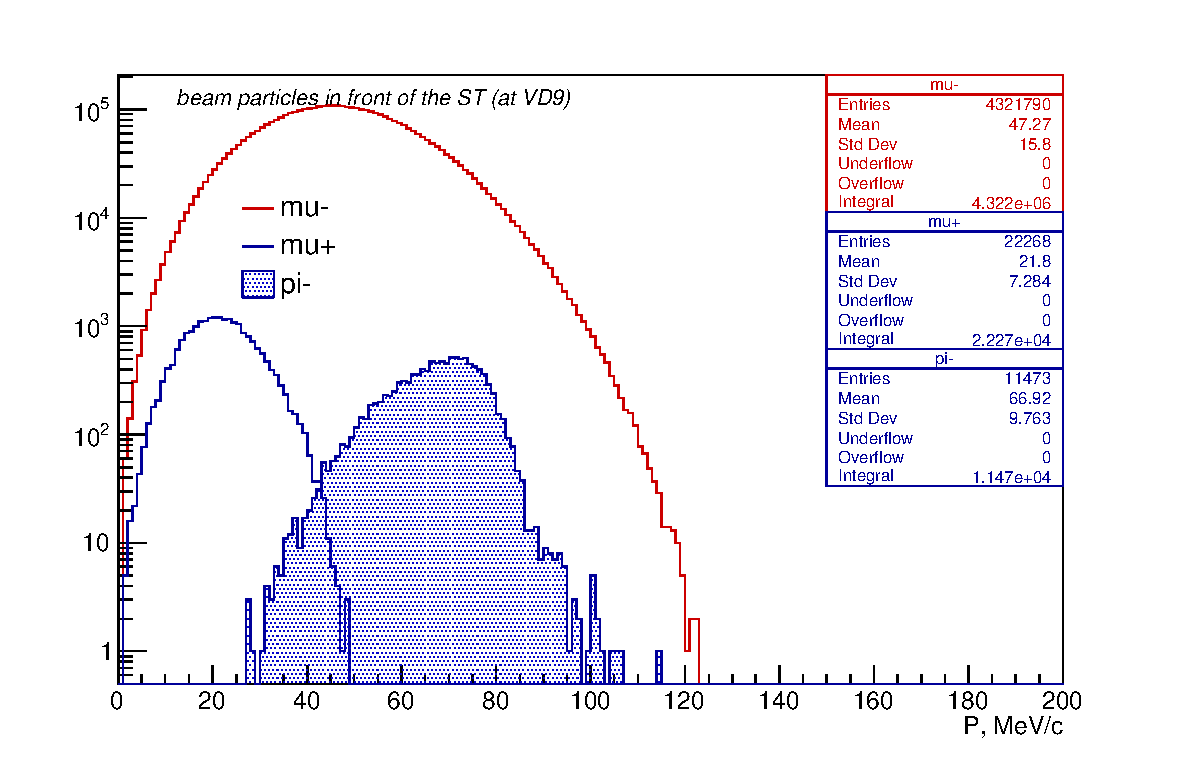
\includegraphics[width=0.54\textwidth]{figures/pdf/figure_03700_bmum0s37b0_vdet_xx09_mom}
      % }
    };
    \node[anchor=south west,inner sep=0] at (10,0.) {
      % \node[shift={(0 cm,0.cm)},inner sep=0,rotate={90}] at (0,0) {}
      % \makebox[\textwidth][c] {
      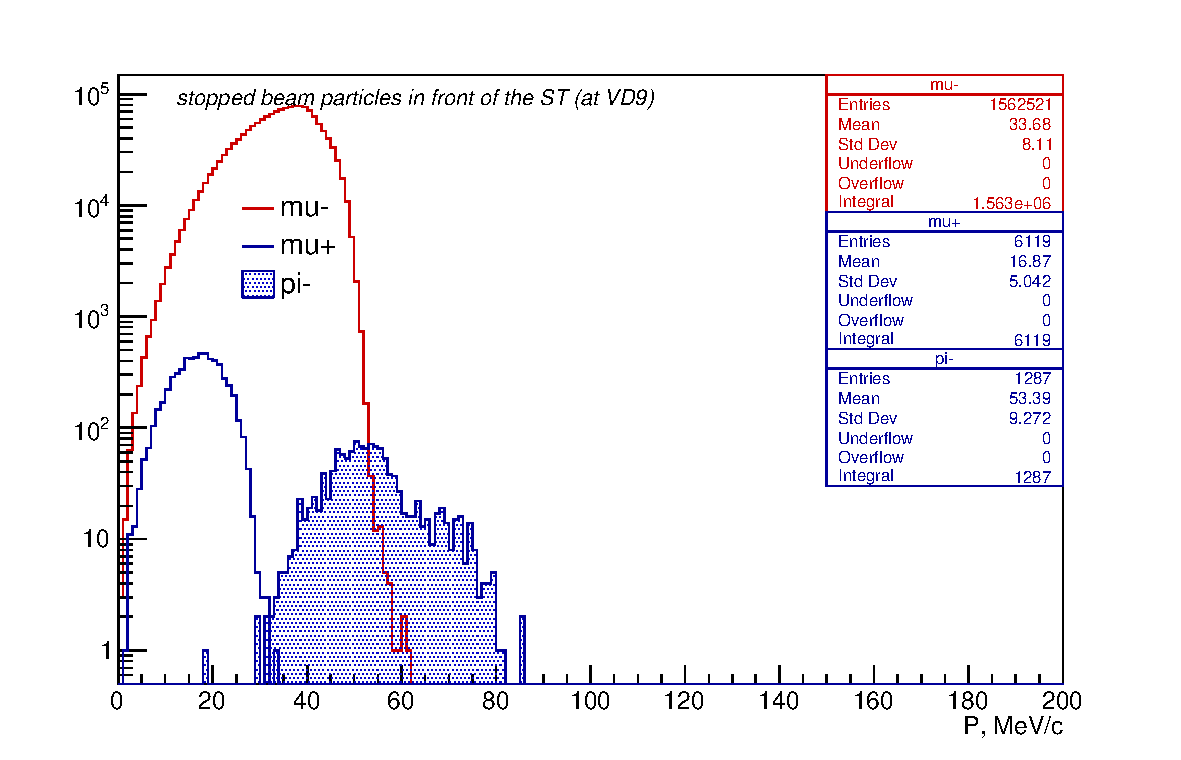
\includegraphics[width=0.54\textwidth]{figures/pdf/figure_03100_bmum0s31b0_vdet_xx09_mom}
      % }
    };
  \end{tikzpicture}
  \caption{
    \label{fig:03700_bmum0s31b0_vdet_xx09_mom}
    a ... 
  }
\end{figure}

\begin{figure}[H]
  \hspace{-0.8in}
  \begin{tikzpicture}
    \node[anchor=south west,inner sep=0] at (0,0.) {
      % \node[shift={(0 cm,0.cm)},inner sep=0,rotate={90}] at (0,0) {}
      % \makebox[\textwidth][c] {
      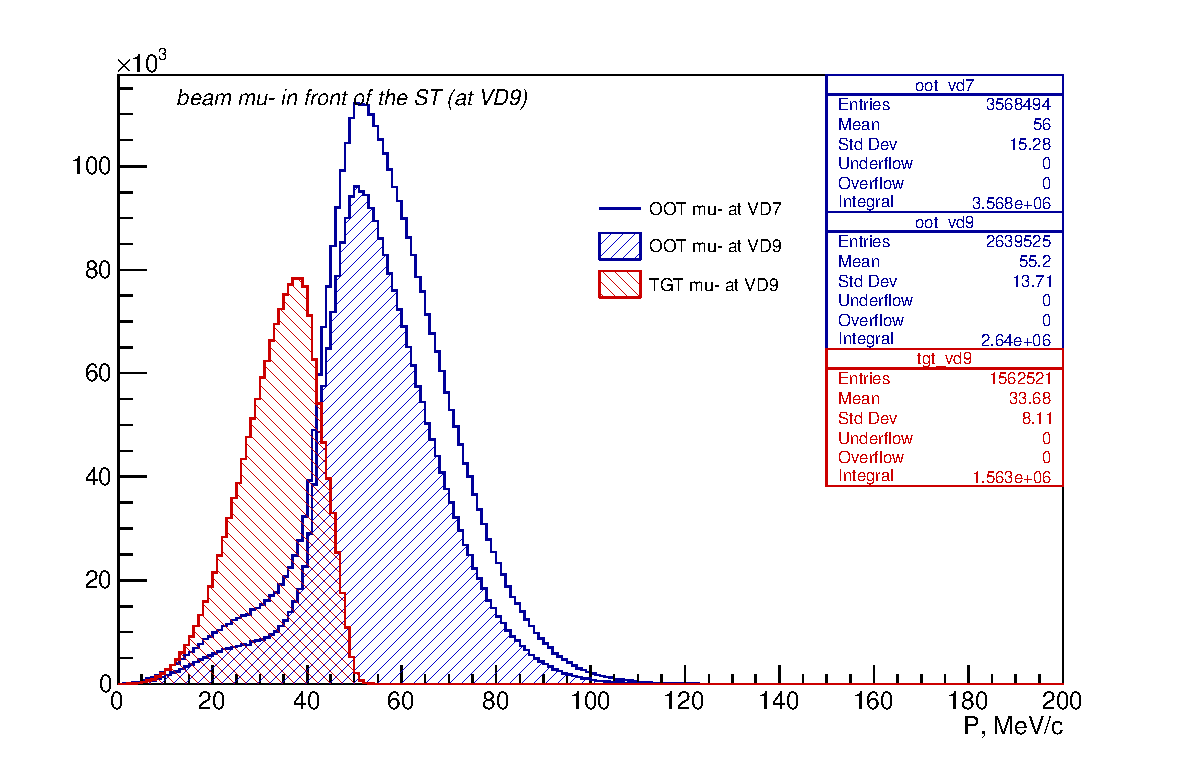
\includegraphics[width=0.80\textwidth]{figures/pdf/figure_03101_bmum0s31b0_vdet_x309_mom}
      % }
    };
    \node[anchor=south west,inner sep=0] at (10,0.) {
      % \node[shift={(0 cm,0.cm)},inner sep=0,rotate={90}] at (0,0) {}
      % \makebox[\textwidth][c] {
      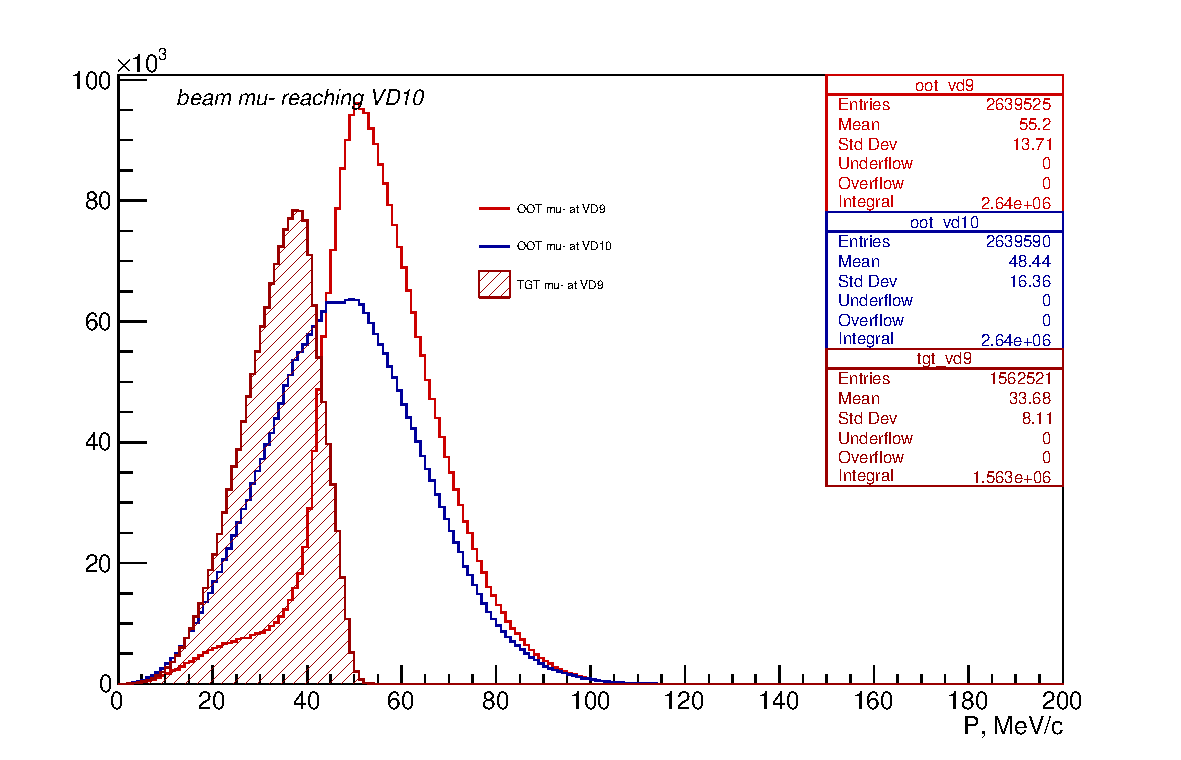
\includegraphics[width=0.80\textwidth]{figures/pdf/figure_03200_bmum0s32b0_vdet_0310_mom}
      % }
    };
  \end{tikzpicture}
  \caption{
    \label{fig:03101_bmum0s31b0_vdet_x309_mom}
    a... 
  }
\end{figure}



%%%%%%%%%%%%%%%%%%%%%%%%%%%%%%%%%%%%%%%%%%%%%%%%%%%%%%%%%%%%%%%%%%%%%%%%%%%%%%
\newpage
\section{Summary}

%%%%%%%%%%%%%%%%%%%%%%%%%%%%%%%%%%%%%%%%%%%%%%%%%%%%%%%%%%%%%%%%%%%%%%%%%%%%%%
%
%%%%%%%%%%%%%%%%%%%%%%%%%%%%%%%%%%%%%%%%%%%%%%%%%%%%%%%%%%%%%%%%%%%%%%%%%%%%%%
\newpage
\bibliographystyle{unsrtnat}
\bibliography{clfv,dio,mu2e_internal_notes}

\end{document}

%%%%%%%%%%%%%%%%%%%%%%%%%%%%%%%%%%%%%%%%%%%%%%%%%%%%%%%%%%%%%%%%%%%%%%%%%%%%%%
% small font sizes: \small \footnotesize \scriptsize \tiny
% ------------------------------------------------------------------------------
% templates
% ------------------------------------------------------------------------------
% Table ~\ref{table:summary} gives summary the numbers used in this study.
%
% \hspace{-0.1in}
% \begin{table}[htbp]
%   \label{table:summary}
%   \begin{center}
%     {\renewcommand{\arraystretch}{1.0}   % change 1.0 to 1.1 to increase the spacing between the table lines
%       \begin{tabular}{|c|c|c|c|}
%         \hline
%                             & default TS geometry & misaligned TS geometry   &  Ratio(default/misaligned)    \\
%         \hline
%         $N_{POT}$            &  $4.96 \cdot 10^6$  &    $5.00 \cdot 10^6$      &   0.992   \\
%         $N_{\mu}^{TS3u}$      &  65648              &     61354                 &   1.070   \\
%         $N_{\mu}^{TS5}$       &  28517              &     27351                 &   1.043   \\
%         $N_{\mu}^{ST}$        &  8868               &      8396                 &   1.056   \\
%         $N_{\mu}^{ST}/N_{POT}$ &  $1.79 \pm 0.02$    &    $1.68 \pm 0.02$        &   $1.065 \pm 0.03$        \\
%         \hline
%       \end{tabular}
%     }
%   \end{center}
%   \caption{
%     Muons rates at different points of the Mu2e beamline and stopping muon rates for nominal and
%     misaligned TS geometries
%   }
%   % \vspace{0.5in}
% \end{table}
